% !TEX program = lualatex
% Build: latexmk (see latexmkrc: LuaLaTeX, biber)
\documentclass[11pt,a4paper]{article}

% ===================================================================== packages
\usepackage{iftex}
\ifPDFTeX
  \PackageError{report}{Compile with LuaLaTeX or XeLaTeX}{}
\fi
\usepackage{fontspec}
\setmonofont{DejaVu Sans Mono}[Scale=MatchLowercase]
\usepackage[british]{babel}
\usepackage{amsmath,amssymb,amsthm,mathtools,bm}
\usepackage[a4paper,margin=2.1cm,headheight=14pt]{geometry}
\usepackage[dvipsnames]{xcolor}
\usepackage{microtype}
\usepackage{csquotes}
\usepackage{booktabs,tabularx,array}
\usepackage{graphicx}
\usepackage{enumitem}
\usepackage[font=small,labelfont=bf,singlelinecheck=off]{caption}
\usepackage{fancyhdr}
\usepackage{titlesec}
\usepackage[most]{tcolorbox}
\usepackage{tikz}
\usetikzlibrary{arrows.meta,positioning,fit,backgrounds,calc,shapes.geometric}
\usepackage[backend=biber,style=authoryear,maxcitenames=2,uniquelist=false,uniquename=false,
            giveninits=true,dashed=false,doi=true,url=false,isbn=false,eprint=false]{biblatex}
\addbibresource{references.bib}
\usepackage[hidelinks]{hyperref}
\usepackage[capitalise,noabbrev]{cleveref}

% ===================================================================== macros
\definecolor{mainblue}{HTML}{1D4E89}
\definecolor{chkgrey}{HTML}{747B86}
\definecolor{specorange}{HTML}{C45C26}
\definecolor{ink}{HTML}{1F2937}
\definecolor{latfill}{HTML}{DAE9FB}
\definecolor{latdraw}{HTML}{4477B5}
\definecolor{obsfill}{HTML}{C9CDD3}
\definecolor{obsdraw}{HTML}{747B86}
\definecolor{platedraw}{HTML}{98A2B3}

\DeclareMathOperator{\Var}{Var}
\DeclareMathOperator{\Cov}{Cov}
\DeclareMathOperator{\tr}{tr}
\DeclareMathOperator{\diag}{diag}
\DeclareMathOperator{\NB}{NB}
\DeclareMathOperator{\Pois}{Poisson}
\newcommand{\E}{\mathbb{E}}
\newcommand{\T}{^{\mkern-1.5mu\mathsf{T}}}
\newcommand{\dd}{\mathrm{d}}
\newcommand{\bmu}{\bm{\mu}}
\newcommand{\bSigma}{\bm{\Sigma}}
\newcommand{\bOmega}{\bm{\Omega}}
\newcommand{\SW}{\bSigma_{W,j}}

% ledger identifier of the machine check behind a statement (Appendix B);
% TODO-Vn markers are replaced by ledger IDs in the last wave
\newcommand{\chk}[1]{\textsf{\scriptsize\color{chkgrey}[#1]}}
% reference not yet in Zotero: printed as plain text in brackets, never a .bib entry
\newcommand{\citeTODO}[1]{\textcolor{chkgrey}{[#1]}}
% link to a DeCovarT vignette (pkgdown site)
\newcommand{\vignette}[2]{\href{https://bastienchassagnol.github.io/DeCovarT/articles/#1}{#2}}
% CardamomOT source file at the pinned commit
\newcommand{\cmfile}[1]{\texttt{\detokenize{#1}}}

\newtcolorbox{answerbox}[1][]{
  colback=mainblue!4!white, colframe=mainblue!75!black, fonttitle=\bfseries\small,
  coltitle=white, colbacktitle=mainblue!90!black, enhanced, fontupper=\small,
  attach boxed title to top left={yshift=-2mm, xshift=5mm}, boxed title style={sharp corners},
  left=4pt, right=4pt, top=4pt, bottom=2pt, #1}
\newtcolorbox{specbox}[1][]{
  colback=specorange!5!white, colframe=specorange!80!black, fonttitle=\bfseries\small,
  coltitle=white, colbacktitle=specorange!90!black, enhanced, fontupper=\small,
  attach boxed title to top left={yshift=-2mm, xshift=5mm}, boxed title style={sharp corners},
  left=4pt, right=4pt, top=4pt, bottom=2pt, title={Speculative}, #1}

\titleformat{\section}{\large\bfseries\color{mainblue}}{\thesection}{0.6em}{}
\titleformat{\subsection}{\normalsize\bfseries}{\thesubsection}{0.5em}{}
\titlespacing*{\section}{0pt}{1.6ex plus .4ex}{0.8ex}
\titlespacing*{\subsection}{0pt}{1.2ex plus .3ex}{0.5ex}
\setlength{\parskip}{0.45ex}
\setlength{\parindent}{0pt}
\setlist{itemsep=1pt,topsep=2pt,leftmargin=1.4em}

\pagestyle{fancy}
\fancyhf{}
\fancyhead[L]{\small\color{chkgrey}DeCovarT and CardamomOT}
\fancyhead[R]{\small\color{chkgrey}\nouppercase{\leftmark}}
\fancyfoot[C]{\small\thepage}
\renewcommand{\headrulewidth}{0.3pt}

% graphical-model styles (RevBayes convention), defined once
\tikzset{
  every node/.style={text=ink},
  const/.style={rectangle, draw=ink, fill=white, minimum size=9mm, line width=0.8pt},
  stoch/.style={circle, draw=latdraw, fill=latfill, minimum size=11mm, line width=0.9pt},
  obs/.style={circle, draw=obsdraw, fill=obsfill, minimum size=11mm, line width=0.9pt},
  det/.style={circle, draw=ink, densely dotted, fill=white, minimum size=11mm, line width=0.9pt},
  var/.style={ellipse, draw=obsdraw, fill=obsfill, minimum height=9mm, inner xsep=2mm, line width=0.9pt},
  plate/.style={draw=platedraw, dashed, rounded corners=5pt, inner sep=4mm, line width=0.8pt},
  platelabel/.style={anchor=north east, font=\small\itshape, text=obsdraw, inner sep=1mm},
  note/.style={font=\small, text=ink!80},
  edge/.style={-{Stealth[length=2.6mm]}, line width=0.8pt, draw=ink}
}
\newcommand{\plate}[3]{%
  \begin{scope}[on background layer]
    \node[plate, fit=#2] (#1) {};
  \end{scope}
  \node[platelabel] (#1-lab) at (#1.south east) {#3};}


\title{\bfseries DeCovarT and CardamomOT:\\ gene selection, noise layers and what a network means}
\author{Bastien Chassagnol\thanks{INSERM. First draft, written with Claude Code (Anthropic). Statements
marked \chk{TODO-Vn} wait for the SymPy ledger of \cref{app:ledger}; none of them is called verified
yet.}}
\date{30 October 2026 (draft)}

\begin{document}
\maketitle
\thispagestyle{fancy}

\begin{abstract}
\noindent DeCovarT \parencite{chassagnolDeCovarTMultidimensionalProbalistic2023} estimates cell-type
fractions from bulk RNA-seq, and models each type by a mean and a gene--gene covariance. CardamomOT
\citeTODO{Maugé \& Ventre 2026, doi:10.1371/journal.pcbi.1014838} infers a signed, directed gene
regulatory network from time-stamped single-cell snapshots, through a mechanistic bursting model. Both
pick a small gene panel from a whole transcriptome, and both estimate a gene--gene structure, but for
opposite reasons: in DeCovarT the covariance is a nuisance that weights genes, in CardamomOT the network
is the estimand. We compare the two along five axes: (i)~gene selection, (ii)~expression versus
measurement model, (iii)~a speculative side axis (convolution, Wiener filter, mean-field ansatz),
(iv)~the diagonal of a network and self-regulation, (v)~how many genes the data can support. The
CardamomOT code at commit \texttt{4a6305c} adds a per-cell depth layer that the paper does not describe,
and its diagnostic is the main item DeCovarT could borrow. CardamomOT could borrow a cell-quality tier,
a held-out likelihood for its penalty, and a within-basin covariance.
\end{abstract}

% =====================================================================
\section{Aims, estimands and the two models side by side}\label{sec:aims}

\textbf{Sources.} CardamomOT: the published paper (PDF pages cited as \enquote{p.}) and the repository
at a fixed commit.\footnote{\url{https://github.com/eliasventre/CardamomOT}, commit
\texttt{4a6305cd3699be7a10d8da97b9ad892e41c90adc}. Files read: \cmfile{estimate_cell_depth.py},
\cmfile{inference/depth.py}, \cmfile{inference/depth_model.py}, \cmfile{inference/gene_selection.py},
\cmfile{inference/gandrillon.py}, \cmfile{inference/network.py}. The repository ships no
\texttt{CITATION.cff}.} Gandrillon's sympathoadrenal study \citeTODO{Gandrillon 2025,
doi:10.1101/2025.03.21.644507} supplies CardamomOT's gene-selection rule. All PDFs were read with local
tools only.

\textbf{Notation.} Genes $g=1,\dots,G$; cell types $j=1,\dots,J$ with $C_j$ reference cells; cells $c$;
bulk samples $i$ with $n_i$ cells; reference UMI counts $x_{gc}$ with size factor $s_c$; fractions
$\bm p_{\cdot i}$. DeCovarT's within-type covariance on the linear count scale is $\SW$, its precision
$\bOmega_j=\SW^{-1}$, the empirical covariance $\bm V_j$. CardamomOT's interaction matrix is
$\bm\theta=(\theta_{gh})$, the influence of gene $h$ on gene $g$ (p.~6). We write the negative binomial
as $\NB(a,r)$, shape $a$ and rate $r$ (the paper writes $\NB(a,b)$, the code $\NB(k,c)$), so that the
mean is $a/r$.

\begin{table}[tbp]
\centering
\caption{The two methods side by side. Page numbers refer to the CardamomOT paper unless a file name is
given; \enquote{code} means the repository at commit \texttt{4a6305c}.}
\label{tab:side}
\footnotesize
\begin{tabularx}{\textwidth}{@{}>{\raggedright\arraybackslash}p{0.13\textwidth}
  >{\raggedright\arraybackslash}X >{\raggedright\arraybackslash}X@{}}
\toprule
 & DeCovarT & CardamomOT \\
\midrule
Data & bulk RNA-seq samples and one reference: sorted populations, or the cells of one specimen
  (Suppinger: single-cell GSE229513, bulk GSE229386, matched at 48\,h) &
  scRNA-seq snapshots at successive time points, raw counts; optional prior network $\bm\theta_0$ and
  degradation rates (p.~8) \\
Estimand & fractions $\bm p_{\cdot i}$ of each bulk sample, with Wald intervals &
  signed directed $\bm\theta$, burst parameters, protein trajectories (pp.~6, 8) \\
Cell-level law & first two moments $(\bmu_j,\SW)$ per type on the linear UMI scale &
  $M_g\mid\bm P\sim\NB$ from promoter bursting; a mixture over promoter basins, genes independent given
  the basin (Eq.~4, p.~7) \\
Aggregate & sum of $n_i$ cells: $\bm y_{\cdot i}\sim\mathcal N\bigl(c_i\sum_jp_{ji}\bmu_j,\;
  \phi_i\sum_jp_{ji}\SW\bigr)$, linear in $\bm p$; population references give
  $\sum_jp_{ji}^2\bSigma_j$, quadratic \chk{TODO-V6} &
  none (no bulk); the population marginal is the basin mixture \\
Noise layers & expression and measurement mixed in $\SW$; bulk scales $c_i$, $\phi_i$ &
  paper: expression (bursting) only; code: per-cell depth factor $s_c$ (\cref{sec:noise}) \\
Gene selection & QC, presence in every type, consistency screen, optional Fisher-information refinement
  (\cref{sec:genes}) & paper: core set plus databases (p.~28); code: entropy and Wasserstein terminals,
  basin separability, coarse network, Steiner closure \\
Role of the network & nuisance plug-in that weights genes (generalised least squares) &
  the object of inference \\
Sparsity & dense shrinkage $\hat\bSigma$ by default; graphical lasso with cross-validated $\lambda$ as
  an alternative & $\ell_1$ towards $\bm\theta_0$ (Eq.~10, p.~9); code: quantile universal threshold
  per target gene, then an adaptive-lasso refinement (\cmfile{network.py}) \\
Diagonal & $\omega_{gg}=1/\Var(x_g\mid\bm x_{-g})$, never penalised &
  $\theta_{gg}$, directed self-regulation; \enquote{no specific penalty} (p.~28) \\
Inference & maximum likelihood, profile likelihood, Wald intervals for $\bm p$ &
  point estimates; run-to-run variability over 3--5 seeds (p.~27) \\
\bottomrule
\end{tabularx}
\end{table}

The two models answer different questions (\cref{tab:side}). DeCovarT is a multivariate regression in
the strict sense: several correlated responses (the genes) share one design (the fractions). Its gene
covariance matters because it weights genes, as in generalised least squares. CardamomOT is a
mechanistic model of the cell, and its network is what the user reads. A good covariance for DeCovarT
need not be a good network for CardamomOT, and the converse also holds (\cref{sec:diag}).

% =====================================================================
\section{Gene selection (axes i and v)}\label{sec:genes}

\subsection{CardamomOT: paper and code}

The paper treats the panel as prior information. \enquote{All experimental applications presented here
operate on gene subsets rather than the full transcriptome (Appendix C), which is not a neutral choice}
(p.~27); \enquote{the selected gene set should be recognised as a form of prior information in its own
right} (p.~27). It recommends a core set of nodes from prior knowledge, completed by curated interaction
databases and a coarse genome-wide network, and calls the automation \enquote{ongoing work} (p.~28). For
Semrau and Kameneva, the applications use gene lists from earlier work; for Schiebinger, markers plus
\enquote{dynamically variable genes} ranked by entropy and Wasserstein distances (p.~32).

The code at \texttt{4a6305c} automates that recommendation (\cmfile{inference/gene_selection.py},
module docstring):
\begin{itemize}
  \item \textbf{gene universe:} mitochondrial, ribosomal-protein and non-coding genes are excluded by name
        or biotype;
  \item \textbf{terminal genes} from Gandrillon's workflow (\cmfile{inference/gandrillon.py}): \enquote{KD}
        is the one-dimensional Wasserstein distance between the counts of a gene at two consecutive time
        points, divided by the gene's standard deviation over the pair; \enquote{MDE} is the absolute
        change of a discrete entropy estimated by the BUB estimator \citeTODO{Paninski 2003, Neural
        Computation, doi to verify}; terminals are then chosen by a round robin over cell types, each
        tested against the rest by a Wilcoxon test on log-normalised counts (Scanpy
        \cmfile{rank_genes_groups}) \citeTODO{Wolf et al.\ 2018, Scanpy, doi to verify};
  \item \textbf{basin separability:} genes whose negative-binomial modes are well separated
        (\cmfile{nb_init_separation});
  \item \textbf{a coarse network} on highly variable genes (OTVelo-Corr);
  \item \textbf{closure:} a budgeted prize-collecting Steiner selection that anchors the terminals to the
        stimuli.
\end{itemize}

\textbf{Gandrillon's criteria.} The \enquote{Kantorovich distance} cited by Gandrillon (p.~7, to Vershik
2006) is the Wasserstein-1 distance, and the code computes it with \cmfile{scipy.stats.wasserstein_distance}.
\enquote{Delta-entropy} is a change of entropy between consecutive time points; the preprint gives no
formula, and the code uses the BUB estimate of the Shannon entropy of the counts. Gandrillon's Figure~3
caption reads: \enquote{The union of those two lists gave us a list of 97 genes}, the two lists having
200 and 376 genes. A union of these lists has at least 376 genes, so the operation that yields 97 genes
is an intersection. The CardamomOT port states it as such: \enquote{union over transitions of the top\_n
KD genes, intersected with the union over transitions of the top\_n MDE genes}. A second count does not
add up either: with five transitions, a union of the top 50 entropy genes per transition has at most
250 genes, not 376. Neither point changes the method; both concern its description. The 97-gene panel
contains ten ribosomal-protein genes and \textit{MT-CYB} (Gandrillon, Table~1), which the current
universe filter would exclude; the CardamomOT paper notes housekeeping genes such as \textit{RPL30} among
the top Kameneva regulators (p.~18).

\subsection{DeCovarT}

The estimand is a gene panel that makes $(\bmu_j,\SW)$ estimable and informative about $\bm p$, not
population-level differential expression. With one specimen, cells are not replicates, so a $p$-value
describes a screen inside that specimen \parencite{zimmermanPracticalSolutionPseudoreplication2021,
squairConfrontingFalseDiscoveries2021}. The tiers are written in the
\vignette{03-1-feature-selection.html}{feature-selection vignette}:
\begin{itemize}
  \item \textbf{QC:} cells by library size, detected genes and mitochondrial fraction; genes by detection;
  \item \textbf{presence in every type}, so that each $\SW$ is non-singular; this also removes perfect
        markers, for which proportions are not identified once gene-wise platform ratios are allowed
        \parencite[p.~7]{xieStatisticalInferenceCell2026};
  \item \textbf{consistency screen} (\enquote{marker gene consistency},
        \textcite[p.~2]{wangBulkTissueCell2019}): the between/within ratio on Pearson residuals, or its
        count-scale versions, the analysis-of-deviance and quasi-likelihood $F$ tests
        \parencite{lundDetectingDifferentialExpression2012}; the test is a gate, and genes are ranked by
        effect size;
  \item \textbf{optional refinement} by the Fisher information for $\bm p$, which needs $\SW$.
\end{itemize}
For two types and one gene, under the single-cell model with equal within-type variances $\sigma_g^2$,
the Fisher information for $p$ is $n_i\Delta_g^2/\sigma_g^2$, with $\Delta_g=\mu_{g1}-\mu_{g2}$
(\cref{app:fisher}) \chk{TODO-V4}. The ANOVA ratio on $C$ cells per type estimates $(C/2)\Delta_g^2/\sigma_g^2$,
so both rank genes alike. With unequal variances or correlated genes they do not: the multivariate
information with a common $\bSigma_W$ is $n_i\bm\Delta\T\bSigma_W^{-1}\bm\Delta$, a Mahalanobis distance.
The Hellinger distance between the two type laws is monotone in that distance; the 2-Wasserstein distance
is not, since for equal covariances it reduces to $\lVert\bm\Delta\rVert$. This links the screen to the
overlap criteria of the \vignette{S6-feature-screening-scenario.html}{screening scenario}.

The two methods push the within-group variance in opposite directions. CardamomOT keeps genes whose
distribution changes in time and splits into separable basins, so multimodality is wanted. DeCovarT
wants a unimodal law within each type, with a covariance it can estimate.

\subsection{How many genes can the data support?}\label{sec:ceiling}

Three thresholds, from the weakest to the strongest:
\begin{itemize}
  \item \textbf{existence:} the graphical lasso with $\lambda>0$, positive empirical variances and an
        unpenalised diagonal has a unique positive-definite solution for any $n\ge2$
        \parencite{carterExistencePenalisedLikelihood2025}; convergence says nothing about the graph;
  \item \textbf{maximum-likelihood threshold} $\mathrm{mlt}(G)$: the smallest $n$ for which the
        unpenalised MLE on a given graph exists almost surely; it equals the largest clique for chordal
        graphs \citeTODO{Uhler 2012, arXiv:1012.2643; Gross \& Sullivant, arXiv:1404.6989}. On graphs
        selected by the graphical lasso with $p\le9$, the MLE never existed at $n=1$, and the probability
        that it exists grows with $n$ and with the penalty \citeTODO{Bernstein \& Outlaw 2023,
        arXiv:2312.03145};
  \item \textbf{support recovery:} $n\gtrsim d^2\log G$, with $d$ the maximum degree, under incoherence
        and minimum-signal conditions \citeTODO{Ravikumar et al.\ 2011, arXiv:0811.3628}.
\end{itemize}
CardamomOT has $G^2$ interaction parameters (\enquote{$10^4$ for $n=100$}, p.~27) and recommends
\enquote{not exceeding of the order of 100 genes in the fully unconstrained setting} (p.~28), with more
genes allowed when $\bm\theta_0$ fixes more entries. DeCovarT faces the same trade-off per type: several
Suppinger types have $C_j<G$, which rules out the unpenalised covariance and puts support recovery out
of reach for all but very sparse graphs. Its plug-in only needs a good $\hat\bSigma$, not the right
graph, which is why dense shrinkage \parencite{schäferShrinkageApproachLargescale2005} is the default.

\textbf{Scalable alternatives.} An edge-weighted graphical lasso takes a penalty matrix
$\bm\Lambda=(\lambda_{gh})$: small weights for whitelisted pairs, zero constraints for blacklisted ones
\parencite{friedmanSparseInverseCovariance2008}. CardamomOT's prior network, or an OmniPath prior as in
its repository (p.~27), can enter DeCovarT this way. Neighbourhood selection fits $G$ lasso regressions
\citeTODO{Meinshausen \& Bühlmann 2006, doi:10.1214/009053606000000281}; it scales well but returns a
graph, not a positive-definite $\hat\bSigma$, so a refit under the selected zeros is needed. A penalty
chosen for prediction does not select the true neighbourhood (their Proposition~1, p.~5), which matters
for CardamomOT, not for DeCovarT's plug-in.

\textbf{Selection removes what it should estimate.} A panel chosen for small within-type variance, such
as ReDeconv's smallest coefficients of variation \parencite[p.~14]{luTranscriptomeSizeMatters2025} or
MuSiC's \enquote{cross-cell consistent genes} \parencite[p.~3]{wangBulkTissueCell2019}, leaves
covariances dominated by Poisson sampling. Their correlations are then attenuated (\cref{sec:noise}),
and the estimated precision looks diagonal for reasons that have nothing to do with regulation.

\begin{answerbox}[title=In short: gene selection]
\begin{itemize}
  \item CardamomOT selects for change in time and multimodality, and treats the panel as prior
        information. DeCovarT selects for between-type separation with an estimable unimodal within-type
        law. The criteria are not interchangeable.
  \item The univariate ANOVA ratio is a screen; the Fisher information for $\bm p$ is the objective.
        They agree for two types only with equal variances and independent genes \chk{TODO-V4}.
  \item Both methods meet the same ceiling: $G^2$ parameters against $C_j$ cells. Prior structure (a
        whitelist, $\bm\theta_0$) is the way to more genes.
\end{itemize}
\end{answerbox}

% =====================================================================
\section{Expression model versus measurement model (axis ii)}\label{sec:noise}

\textcite[p.~3]{sarkarSeparatingMeasurementExpression2021} separate \enquote{a measurement model
[\ldots] the conditional distribution $p(X\mid\Lambda)$} from \enquote{a model for the expression levels
$p(\Lambda)$}. For UMI data, Poisson measurement suffices: $x_{gc}\mid\lambda_{gc}\sim
\Pois(x_{c+}\lambda_{gc})$, and gene--gene correlation belongs to the expression model.
\textcite{fangExtrinsicBiologicalStochasticity2025} add a cell-wide factor $c=c_{\mathrm{tech}}c_{\mathrm{bio}}$
that multiplies the mean of every gene (their eqs~1--2, pp.~3--4). For intrinsically uncorrelated genes,
the normalised covariance $\Cov(X_a,X_b)/(\E X_a\E X_b)$ then equals the extrinsic noise
$\Var c/(\E c)^2$ (eq.~5, p.~5). They estimate it by the mode of the normalised covariances, call
\enquote{Poisson genes} those whose bootstrap interval of normalised variance contains it, and take the
Poisson MLE of the size factor on those genes (p.~16). Normalising by size factors \enquote{can eliminate
biological stochasticity present in extrinsic \enquote{noise}} (p.~2).

\begin{figure}[tbp]
\centering
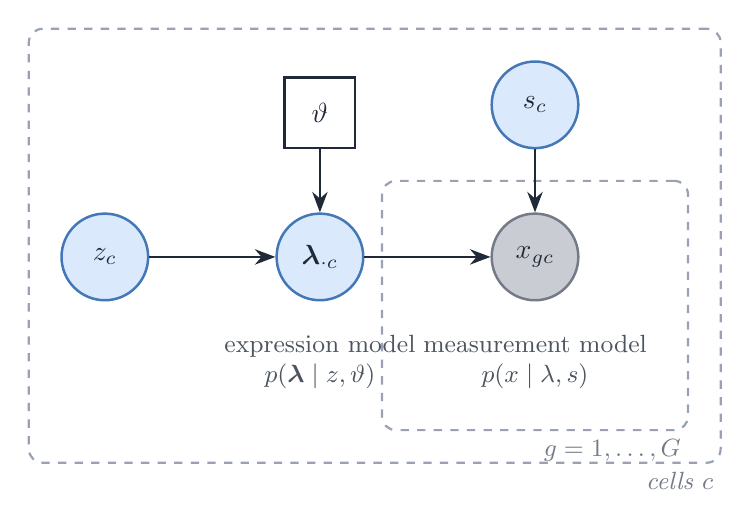
\begin{tikzpicture}[node distance=9mm and 16mm]
  \node[stoch] (z) {$z_c$};
  \node[stoch, right=of z] (lam) {$\bm\lambda_{\cdot c}$};
  \node[const, above=8mm of lam] (par) {$\vartheta$};
  \node[obs, right=of lam] (x) {$x_{gc}$};
  \node[stoch, above=8mm of x] (s) {$s_c$};
  \node[note, below=3mm of lam, align=center] (nexp) {expression model\\$p(\bm\lambda\mid z,\vartheta)$};
  \node[note, below=3mm of x, align=center] (nmeas) {measurement model\\$p(x\mid\lambda,s)$};
  \draw[edge] (z) -- (lam);
  \draw[edge] (par) -- (lam);
  \draw[edge] (lam) -- (x);
  \draw[edge] (s) -- (x);
  \plate{genes}{(x)(nmeas)}{$g=1,\ldots,G$}
  \plate{cells}{(z)(lam)(s)(genes)(nexp)}{cells $c$}
\end{tikzpicture}
\caption{The two noise layers for one reference cell. $z_c$ is the label (cell type $j$ in DeCovarT,
promoter basin in CardamomOT), $\vartheta$ the parameters ($\bmu_j,\SW$ in DeCovarT; NB shapes and rates
in CardamomOT), $s_c$ the depth factor. CardamomOT's paper models $\bm\lambda\mid z$ as a product of
independent NB laws and omits $s_c$; its code adds $s_c$. DeCovarT estimates the covariance of $x$
directly, so both layers enter $\SW$.}
\label{fig:layers}
\end{figure}

\textbf{CardamomOT, paper.} The negative binomial comes from bursting and is an expression model
(p.~6). No size factor, library size or capture term appears in Eqs~3--4; technical noise is examined
only as a robustness test with simulated binomial dropout of 5--90\,\% (p.~17).

\textbf{CardamomOT, code at \texttt{4a6305c}.} The measurement layer is a per-cell depth factor $s_c$
(\cmfile{estimate_cell_depth.py}, \cmfile{inference/depth.py}, \cmfile{inference/depth_model.py}).
\begin{itemize}
  \item \textbf{Rationale} (script docstring): a depth common to all genes of a cell \enquote{acts like a
        hidden common regulator: it correlates all genes and can move cells between NB basins}.
  \item \textbf{Estimation} within homogeneous groups (sample, time, cell type), on the whole transcriptome
        (at least 10{,}000 genes, otherwise nothing is estimated); the library size leaves out the 50 most
        expressed genes. The default method, \texttt{poissonian}, follows Fang \& Pachter: extrinsic noise
        as the mode of normalised covariances, iterated Poisson genes, $s_c$ as the Poisson MLE on those
        genes, then a pairwise least-squares rescaling between groups. The alternative,
        \texttt{group\_median}, divides the library size by the group median.
  \item \textbf{How it enters:} with the default \texttt{depth\_model = 'mean'}, counts are
        $\NB(a,r/s_c)$ (code: $\NB(k,c/s_i)$): depth multiplies the mean and leaves the shape $a$
        unchanged, as in scVI. The option \texttt{'burst\_frequency'} uses $\NB(a s_c,r)$. Counts stay
        integers; $s_c$ is stored in \texttt{obs['depth\_factor']} and \texttt{X} is untouched.
  \item \textbf{When it is applied:} the diagnostic recommends the correction if the depth share of the
        mean within-group pairwise correlation exceeds 0.5, or if more than half of the genes have NB modes
        closer than the depth spread. The correlation share is computed on the log1p counts of 1{,}000
        reference genes (the most variable among genes detected in more than 5\,\% of cells), with and
        without the log library size regressed out. The depth spread is the median over groups of
        $q_{0.95}/q_{0.05}$ of $s_c$. The correction is written only if the user allows it.
  \item \textbf{No cell or gene is removed for abnormal depth.} There is no MAD or quantile filter. Cells
        flagged as doublets are counted and reported, never filtered; a warning recommends upstream
        removal when depth correlates with the doublet score above 0.3.
\end{itemize}

\textbf{DeCovarT.} $\SW$ estimated from raw UMI counts mixes both layers. If
$x_{gc}\mid\bm\lambda_{\cdot c},s_c\sim\Pois(s_c\lambda_{gc})$ with $s_c$ independent of $\bm\lambda_{\cdot c}$
within type $j$, the law of total covariance gives (\cref{app:depth})
\begin{equation}\label{eq:depth}
\Cov(\bm x_{\cdot c})=\E(s^2)\,\bSigma^{\lambda}_j+\Var(s)\,\bmu^{\lambda}_j\bmu^{\lambda\mathsf T}_j
+\E(s)\diag(\bmu^{\lambda}_j).
\end{equation}
\begin{itemize}
  \item \textbf{Depth} adds a rank-one term along the mean $\bmu^{\lambda}_j$, common to all gene pairs.
        Its biological part (cell size, the $S_j$ of DeCovarT's estimand) aggregates into the bulk and is
        wanted. Its technical part (capture) does not reach the bulk. Because the term lies along the
        type means, an inflated technical share down-weights the very directions that separate the types
        (our reading, not tested). Splitting the two parts needs controls such as spike-ins or ambient
        transcripts \parencite[pp.~8--11]{fangExtrinsicBiologicalStochasticity2025}; CardamomOT's
        diagnostic measures the total depth share only.
  \item \textbf{Poisson sampling} adds to the diagonal only, so it attenuates every correlation and makes
        lowly expressed panels look independent.
  \item \textbf{Bulk scales} $c_i=a_in_i$ and $\phi_i=a_i^2n_i$ absorb a platform scale per bulk sample;
        they do not remove the cell-level depth variance from $\SW$.
  \item \textbf{A model that separates the layers:} the Poisson log-normal, $x_{gc}\sim\Pois(s_c
        e^{z_{gc}})$ with $\bm z_{\cdot c}\sim\mathcal N(\bmu_z,\bSigma_z)$
        \parencite{chiquetPoissonLognormalModelVersatile2021}. Its offset is the measurement layer and
        $\bSigma_z$ the expression layer. Mapped back to the linear scale,
        $\E\bm x=s\,e^{\bmu_z+\diag(\bSigma_z)/2}$ and $\Cov\bm x=\diag(\E\bm x)+(\E\bm x\,\E\bm x\T)\circ
        (e^{\bSigma_z}-1)$ for fixed $s$ \chk{TODO-V3}.
\end{itemize}

\begin{answerbox}[title=In short: noise layers]
\begin{itemize}
  \item In the paper, CardamomOT's NB is an expression model with no measurement layer. The code at
        \texttt{4a6305c} adds one: a per-cell depth $s_c$ that multiplies the NB mean, applied only when
        depth explains more than half of the within-group correlation or blurs the NB basins. It removes
        no cell and no gene; doublets are only flagged.
  \item DeCovarT's $\SW$ contains a rank-one depth term and a Poisson diagonal. The biological share of
        depth should stay, the technical share should not.
  \item DeCovarT can run the depth-share diagnostic on Suppinger before estimating $\SW$. Cell QC stays a
        separate tier, which CardamomOT does not perform.
\end{itemize}
\end{answerbox}

% =====================================================================
\section{The diagonal and self-regulation (axis iv)}\label{sec:diag}

\textbf{Two different objects.} In a Gaussian graphical model, $\omega_{gg}=1/\Var(x_g\mid\bm x_{-g})$ is a
conditional precision, and an edge is a non-zero partial correlation $-\omega_{gh}/\sqrt{\omega_{gg}
\omega_{hh}}$. The diagonal is never an edge. In CardamomOT, $\theta_{gg}$ enters the activation rate of
gene $g$ through its own protein (Eq.~1, p.~6): a directed self-loop.

\textbf{Self-activation and bistability.} \enquote{The combination of a positive auto-activation with a
negative basal parameter $\beta_i$ is the most parsimonious way to produce bistability for an isolated
gene} (p.~28). This is the autocatalytic case of \citeTODO{Ferrell 2002,
doi:10.1016/S0955-0674(02)00314-9}: bistability needs feedback, \enquote{some type of non-linearity
within the feedback circuit}, and balanced legs (p.~3 of that review). CardamomOT reports diagonal
coefficients \enquote{systematically non-negligible across all three datasets} (p.~18).

\textbf{Linking the two through the stationary covariance.} Around one basin, linearise the dynamics as
an Ornstein--Uhlenbeck process $\dd\bm x=\bm A(\bm x-\bm x^\ast)\dd t+\bm B\,\dd\bm W$. The stationary
covariance solves the Lyapunov equation $\bm A\bSigma+\bSigma\bm A\T+\bm Q=\bm 0$, $\bm Q=\bm B\bm B\T$.
Write $a_g=d_g-\varsigma_g>0$ for the net decay of gene $g$: degradation minus linearised
self-activation. For two genes with $1\to2$ of strength $b$ (\cref{app:lyap}),
\begin{equation}\label{eq:lyap2}
\sigma_{11}=\frac{q_1}{2a_1},\qquad \sigma_{12}=\frac{b\,q_1}{2a_1(a_1+a_2)},\qquad
\omega_{12}=-\frac{2a_2(a_1+a_2)\,b}{(a_1+a_2)^2q_2+b^2q_1}\quad\chk{TODO-V5}.
\end{equation}
\begin{itemize}
  \item Self-activation acts only through $a_g$: a larger $\varsigma_g$ inflates $\sigma_{gg}$ and the
        conditional variance, so it lowers $\omega_{gg}$. It appears nowhere as a \enquote{self-edge}.
  \item $\omega_{12}\neq0$ if and only if $b\neq0$, but its sign and size mix $b$ with the decays and noise
        intensities, and the direction is lost.
  \item With three genes, a fork $1\to2$, $1\to3$ gives $\omega_{23}\propto-b_{21}b_{31}\neq0$: two
        co-regulated targets are linked in the precision although neither regulates the other
        \chk{TODO-V5}. A static structural equation model with the same fork would give $\omega_{23}=0$.
  \item The linear model has one basin. Bistability requires the non-linearity that the linearisation
        removes, and produces a bimodal law within a cell type, which a Gaussian within-type law cannot
        represent. DeCovarT's counterpart of a basin is a subtype: more components in the convolution.
\end{itemize}

\textbf{Penalising the diagonal.} When the graphical lasso penalises every entry, its covariance estimate
has $\hat W_{gg}=V_{gg}+\lambda$ \parencite{friedmanSparseInverseCovariance2008}: every variance is biased
upwards by $\lambda$. DeCovarT's likelihood uses those variances as gene weights, so the diagonal is
never penalised (\texttt{penalize.diagonal = FALSE}). For CardamomOT, the diagonal penalty is a prior
choice. The paper says \enquote{we deliberately choose not to apply a specific penalty on diagonal
coefficients} (p.~28), and suggests zeroing entries of $\bm\theta_0$ when auto-regulation is implausible.
Eq.~10 penalises $\bm\theta-\bm\theta_0$ entrywise. In the code (\cmfile{network.py}), the first
$\ell_1$ step penalises the self-loop like any edge inside the prior support, and the adaptive-lasso
refinement leaves \enquote{self-regulation and basals unpenalized} (\cmfile{refine_inference}). Stating
that two-stage rule in the paper would remove an ambiguity.

\begin{answerbox}[title=In short: diagonal]
\begin{itemize}
  \item $\omega_{gg}$ is a conditional precision; $\theta_{gg}$ is a directed self-loop. They are related
        only through the stationary covariance of a linearised model, where self-activation lowers
        $\omega_{gg}$ \chk{TODO-V5}.
  \item A precision edge is not a regulatory edge: a fork creates one without a direct link.
  \item Never penalise the GGM diagonal in DeCovarT. In CardamomOT the self-loop penalty is a prior
        choice, which the code makes differently in its two stages.
\end{itemize}
\end{answerbox}

% =====================================================================
\section{A side axis (iii): convolution, Wiener filter, mean field}\label{sec:side}

\begin{specbox}
These are analogies to explore, not results. Only the Wiener--BLUP identity is a derivation.
\begin{itemize}
  \item \textbf{Convolution and characteristic functions.} The bulk is a sum of independent cell
        profiles, so its density is a convolution, and its characteristic function is a product:
        $\varphi_{\bm y}(\bm t)=\prod_j\varphi_{\bm x_j}(p_j\bm t)$ for population references, or
        $\varphi_{\mathrm{cell}}(\bm t)^{n_i}$ given a mixture over types for single-cell references
        (\cref{app:conv}). DeCovarT's Gaussian is the central-limit form of that product. For a
        non-Gaussian cell law, such as a fitted CardamomOT NB mixture, the bulk law of one gene could be
        computed by FFT on the count lattice \citeTODO{Cooley \& Tukey 1965, doi to verify}. In several
        dimensions the lattice grows exponentially, so this stays a check for a few genes.
  \item \textbf{Wiener filter as BLUP.} Writing $\bm x_{\cdot j,i}=\bmu_j+\bm\varepsilon_{j}$ with
        $\bm\varepsilon_j\sim\mathcal N(\bm 0,\bSigma_j)$ makes $\bm y=\bmu\bm p+\sum_jp_j\bm\varepsilon_j+\bm e$
        a linear mixed model whose random-effect design depends on $\bm p$. Its marginal covariance is
        $\sum_jp_j^2\bSigma_j+\bm D$, the best linear unbiased predictor of $\bm\varepsilon_j$ is the
        Wiener filter of the DeCovarT article, and maximum likelihood is DeCovarT's fit
        (\cref{app:blup}) \chk{TODO-V1}. REML is then an option, and no full Bayesian treatment is needed.
  \item \textbf{Mean field.} Hartree's ansatz writes a many-particle wave function as a product of
        one-particle functions, each in the average field of the others \citeTODO{Hartree 1928; Fock 1930}.
        CardamomOT's product over genes given the basin is of that kind: genes interact only through the
        basin label and the protein field. DeCovarT's independent cells are another product ansatz. In
        both, the neglected correlation (Fock's exchange term in physics) is the within-basin covariance
        that CardamomOT reports losing (p.~12).
\end{itemize}
\end{specbox}

% =====================================================================
\section{What each method could borrow}\label{sec:borrow}

\textbf{DeCovarT from CardamomOT.}
\begin{itemize}
  \item \textbf{The depth-share diagnostic}, run on Suppinger per (time, cell type) before $\SW$ is
        estimated. A large share calls for a decision on the technical part of \cref{eq:depth}, not for
        blind normalisation, since the biological part reaches the bulk.
  \item \textbf{Prior networks as penalty weights} (OmniPath, as in the CardamomOT repository), entering
        an edge-weighted graphical lasso.
  \item \textbf{A basin-separability check} within each type: a gene with separated NB modes inside a type
        signals a subtype that a Gaussian within-type law misrepresents.
  \item \textbf{The panel-as-prior stance} (p.~27): report the panel as part of the model, with the
        sensitivity of $\hat{\bm p}$ to it.
\end{itemize}

\textbf{CardamomOT from DeCovarT.}
\begin{itemize}
  \item \textbf{A cell-quality tier} separate from the depth model: the code removes no cell, and
        Gandrillon's only cell filter was a Scrublet score below 0.2 (his p.~4).
  \item \textbf{A within-basin covariance.} The basin mixture implies a gene covariance that is diagonal
        plus a between-basin term of rank at most $K-1$ for $K$ basins, by the law of total covariance;
        the attenuation of the strongest correlations (p.~12) is the missing within-basin part. A Gaussian
        copula or a Poisson log-normal layer within each basin would restore it.
  \item \textbf{A held-out likelihood for the penalty}, next to the quantile universal threshold. The
        expected Gaussian negative log-score $\tfrac12\{\log\det\bSigma+\tr(\bSigma^{-1}\bSigma_{\mathrm{true}})\}$
        is minimised at $\bSigma=\bSigma_{\mathrm{true}}$ whatever the law of the cells \chk{TODO-V2}, and
        cross-validation estimates the Kullback--Leibler risk for penalised estimators as well
        \parencite{commengesDynamicalBiostatisticalModels2015}; \citeTODO{Commenges et al.\ 2012,
        arXiv:1206.1753} give a fast approximation.
  \item \textbf{An information criterion for the panel}, aimed at the estimand $\bm\theta$ rather than at
        marginal change in time.
  \item \textbf{Uncertainty for $\bm\theta$} beyond seed-to-seed variability, for instance a bootstrap
        over cells within time points.
\end{itemize}

\printbibliography[heading=bibintoc]

% =====================================================================
\clearpage
\appendix
\section{Derivations}\label{app:derivations}

\paragraph{A.1 Two-gene Lyapunov equation.}\label{app:lyap} With $\bm A=\begin{psmallmatrix}-a_1&0\\
b&-a_2\end{psmallmatrix}$ and $\bm Q=\diag(q_1,q_2)$, the three distinct entries of $\bm A\bSigma+\bSigma
\bm A\T+\bm Q=\bm 0$ read $-2a_1\sigma_{11}+q_1=0$, $b\sigma_{11}-(a_1+a_2)\sigma_{12}=0$ and
$2b\sigma_{12}-2a_2\sigma_{22}+q_2=0$. Hence $\sigma_{11}$ and $\sigma_{12}$ as in \cref{eq:lyap2} and
$\sigma_{22}=\{a_1(a_1+a_2)q_2+b^2q_1\}/\{2a_1a_2(a_1+a_2)\}$. Inverting gives
\[
\omega_{11}=\frac{2\{a_1(a_1+a_2)^2q_2+(a_1+a_2)b^2q_1\}}{q_1\{(a_1+a_2)^2q_2+b^2q_1\}},\qquad
\omega_{22}=\frac{2a_2(a_1+a_2)^2}{(a_1+a_2)^2q_2+b^2q_1},
\]
and $\omega_{12}$ of \cref{eq:lyap2}. For the fork $1\to2$ (strength $b$), $1\to3$ (strength $c$),
$\omega_{23}=-4a_2a_3bc\,q_1(a_1+a_2)(a_1+a_3)(a_2+a_3)/\mathcal D$ with $\mathcal D>0$ a polynomial in the
rates and noise intensities \chk{TODO-V5}. These forms come from an exploratory SymPy run, not yet from the
ledger.

\paragraph{A.2 Gaussian convolution.}\label{app:conv} Population references: $\bm y=\sum_jp_j\bm x_j$ with
independent $\bm x_j\sim\mathcal N(\bmu_j,\bSigma_j)$ gives $\varphi_{\bm y}(\bm t)=\prod_j\varphi_{\bm
x_j}(p_j\bm t)=\exp\{i\bm t\T\sum_jp_j\bmu_j-\tfrac12\bm t\T(\sum_jp_j^2\bSigma_j)\bm t\}$, hence the
quadratic covariance. Single-cell references: given $m_j$ cells of type $j$, the sum has mean
$\sum_jm_j\bmu_j$ and covariance $\sum_jm_j\SW$; with $m_j\approx n_ip_j$ and the platform scale $a_i$,
the covariance is $\phi_i\sum_jp_j\SW$, linear in $\bm p$ \chk{TODO-V6}.

\paragraph{A.3 Wiener filter as BLUP.}\label{app:blup} Stack $\bm u=(\bm\varepsilon_1,\dots,\bm\varepsilon_J)$
with $\bm G=\operatorname{blockdiag}(\bSigma_j)$ and $\bm Z=(p_1\bm I_G,\dots,p_J\bm I_G)$. Then
$\bm y=\bmu\bm p+\bm Z\bm u+\bm e$, $\bm e\sim\mathcal N(\bm 0,\bm D)$, and $\bm V=\Var\bm y=\bm Z\bm G\bm
Z\T+\bm D=\sum_jp_j^2\bSigma_j+\bm D$. The BLUP is $\hat{\bm u}=\bm G\bm Z\T\bm V^{-1}(\bm y-\bmu\bm p)$,
whose block $j$ is $p_j\bSigma_j\bm V^{-1}(\bm y-\bmu\bm p)$: the Wiener filter of the DeCovarT article
(\S\,Wiener filter), equal to the posterior mean in the Gaussian model \chk{TODO-V1}.

\paragraph{A.4 ANOVA ratio and Fisher information, $J=2$.}\label{app:fisher} One gene, single-cell model:
$y\sim\mathcal N(c\{p\mu_1+(1-p)\mu_2\},\,\phi\{p\sigma_1^2+(1-p)\sigma_2^2\})$. For $\mathcal N(m(p),v(p))$,
$I(p)=m'(p)^2/v+\tfrac12\{v'(p)/v\}^2$, so $I(p)=c^2\Delta^2/v+\tfrac12\{(\sigma_1^2-\sigma_2^2)/
(p\sigma_1^2+(1-p)\sigma_2^2)\}^2$. If $\sigma_1^2=\sigma_2^2=\sigma^2$, the second term vanishes and
$I(p)=(c^2/\phi)\Delta^2/\sigma^2=n_i\Delta^2/\sigma^2$, since $c^2/\phi=n_i$. With $C$ reference cells per
type, the ANOVA ratio estimates $(C/2)\Delta^2/\sigma^2$, so $I(p)\approx(2n_i/C)\,F$. Over independent genes
the informations add; with correlated genes they do not \chk{TODO-V4}. Under the population model, $v(p)=
p^2\sigma_1^2+(1-p)^2\sigma_2^2$ depends on $p$ even when $\sigma_1=\sigma_2$, and the proportionality fails.

\paragraph{A.5 Depth and sampling in the within-type covariance.}\label{app:depth} Conditionally on
$(\bm\lambda,s)$, counts are independent Poisson with means $s\bm\lambda$. Then $\E\bm x=\E(s)\bmu^\lambda$
and $\Cov\bm x=\E\{\Cov(\bm x\mid\bm\lambda,s)\}+\Cov\{\E(\bm x\mid\bm\lambda,s)\}=\E(s)\diag(\bmu^\lambda)+
\Cov(s\bm\lambda)$, with $\Cov(s\bm\lambda)=\E(s^2)\bSigma^\lambda+\Var(s)\bmu^\lambda\bmu^{\lambda\mathsf T}$
when $s$ and $\bm\lambda$ are independent; this is \cref{eq:depth}. Dividing the off-diagonal terms by
the means recovers Fang \& Pachter's normalised covariance $\Var(s)/(\E s)^2$ for genes with
$\Sigma^\lambda_{gh}=0$, up to the normalisation $\E s=1$.

% =====================================================================
\section{Verification ledger}\label{app:ledger}

The SymPy checks V1--V6 are written last, after every other task of the plan. Until then each statement
that depends on one carries a \chk{TODO-Vn} marker. V1: LMM covariance and BLUP $=$ Wiener filter; V2:
Stein's loss minimised at the true covariance; V3: Poisson log-normal moment map; V4: Fisher information
against the ANOVA ratio for $J=2$; V5: two-gene Lyapunov covariance and precision, fork precision; V6:
single-cell linear against population quadratic covariance at $J=2$.

\IfFileExists{verification-ledger.tex}{\input{verification-ledger.tex}}{\textit{Ledger pending.}}

% =====================================================================
\section{Gene selection in second-generation deconvolution methods}\label{app:review}

\Cref{tab:review} summarises the review behind \cref{sec:genes}. Pages are PDF pages of the local files
(main text unless \enquote{S} for the supplement); a dash means not reported in the parts we extracted.

\begin{table}[htbp]
\centering
\caption{Gene and cell selection in deconvolution methods, and CardamomOT for comparison. QC: quality
control; WLS: weighted least squares; GLS: generalised least squares.}
\label{tab:review}
\scriptsize
\begin{tabularx}{\textwidth}{@{}>{\raggedright\arraybackslash}p{0.11\textwidth}
  >{\raggedright\arraybackslash}p{0.12\textwidth} >{\raggedright\arraybackslash}X
  >{\raggedright\arraybackslash}p{0.15\textwidth} >{\raggedright\arraybackslash}p{0.14\textwidth}
  >{\raggedright\arraybackslash}p{0.12\textwidth}@{}}
\toprule
Method & Cell QC & Gene filter and marker rule & Cross-platform & Weighting & Gene correlation \\
\midrule
RNA-Sieve \parencite{erdmann-phamLikelihoodbasedDeconvolutionBulk2021} & optional: library size
  $\ge3$ MAD from the median (S p.~3) & $\ge20\,\%$ non-zero in one type (S p.~3); bulk outside a
  sub-Gaussian range, MAD outliers on four statistics (eqs~12--13, p.~11) & range bound on the bulk &
  asymptotic Gaussian composite likelihood & ignored \\
DECALS \parencite{caiStatisticalInferenceCelltype2024} & -- & CIBERSORTx S-mode genes $\cap$ Fisher-exact
  markers (p.~13; S pp.~18--19) & -- & constrained OLS/GLS & type covariances, least squares and SCAD
  thresholding (p.~9) \\
MEAD \parencite{xieStatisticalInferenceCell2026} & -- & --; \enquote{not identified if all genes are
  perfect marker genes} (p.~7) & gene-specific platform ratios with mean 1 (pp.~5--6) & diagonal weights,
  sandwich & dependence set by multiple testing \\
ReDeconv \parencite{luTranscriptomeSizeMatters2025} & -- & $t$-test $p<0.05$ against every other type,
  no FDR; fold change $\ge2$; smallest CV; about 100 genes per type (p.~14) & TPM/FPKM on bulk only
  (p.~2) & Gaussian (CLT), heteroscedastic & independent genes \\
MuSiC \parencite{wangBulkTissueCell2019} & -- & all genes by default (p.~7); low within-cluster
  variance in tree-guided stages (pp.~3, 8) & gene- and subject-specific intercept (p.~7) & W-NNLS,
  cross-subject variance (Eq.~10, p.~7) & diagonal \\
deMixSC \parencite{guoDeMixSCDeconvolutionFramework2023} & $<500$ UMI, $<200$ genes, $>50\,\%$
  mitochondrial (p.~11) & bulk vs pseudo-bulk paired $t$-test, BH (pp.~4, 12) & discrepant genes
  down-weighted by $a=1000$ (p.~12) & WLS & diagonal \\
BayesPrism \parencite{chuCellTypeGeneExpression2022} & -- & ribosomal, mitochondrial (pp.~14, 19) and
  chrX/Y genes removed (p.~14); optional scran markers (p.~14) & weak fold-change prior & Bayesian
  multinomial & sum constraint only (our reading) \\
DWLS \parencite{tsoucasAccurateEstimationCelltype2019} & -- & MAST hurdle FDR $<0.01$, log2 FC $>0.5$;
  smallest condition number (p.~7) & -- & WLS, dampening constant by cross-validation (p.~7) & diagonal \\
SCDC \parencite{dongSCDCBulkGene2021} & -- & -- & several references & maximal-variance weights, clipped
  at the 15th/85th percentiles (p.~10) & diagonal \\
RCTD \parencite{cableRobustDecompositionCell2022a} & -- & -- & gene-wise platform random effect (pp.~3, 6)
  & Poisson--lognormal GLMM & -- \\
CardamomOT (code) & none removed; doublets flagged & mitochondrial, ribosomal, non-coding excluded; W1
  and entropy terminals; Wilcoxon round robin; NB separability; Steiner closure & not applicable (no
  bulk) & NB-mixture likelihood & none within a basin (p.~12) \\
\bottomrule
\end{tabularx}
\end{table}

\end{document}
